%%%%%%%%%%%%%%%%%%%%%%%%%%%%%%%%%%%%%%%%%%%%
% IEEE Conference Template 
% Prepared by Dr. Rhio Sutoyo, S.Kom., M.Sc.
% Bina Nusantara University
%%%%%%%%%%%%%%%%%%%%%%%%%%%%%%%%%%%%%%%%%%%%

\documentclass[conference]{IEEEtran}
\IEEEoverridecommandlockouts
% The preceding line is only needed to identify funding in the first footnote. If that is unneeded, please comment it out.
\usepackage{cite}
\usepackage{amsmath,amssymb,amsfonts}
\usepackage{graphicx}
\usepackage{textcomp}
\usepackage{xcolor}
\usepackage{lipsum}
\usepackage{tikz}
\usepackage{float}
\usetikzlibrary{shapes.geometric, arrows.meta, positioning}
 
\def\BibTeX{{
\rm B\kern-.05em{\sc i\kern-.025em b}\kern-.08em
    T\kern-.1667em\lower.7ex\hbox{E}\kern-.125emX}}

\usepackage{algorithm}
\usepackage{algpseudocode}

\begin{document}

\title{Enhancing YouTube ClickBait Detection System Using VADER, Sentence-BERT, and Random Forest\\
}
 
\author{\IEEEauthorblockN{1\textsuperscript{st} Yonathan Eivan Riyadi}
\IEEEauthorblockA{\textit{Computer Science Department, School of Computer Science} \\
\textit{Bina Nusantara University}\\
Jakarta, Indonesia \\
yonathan.riyadi@binus.ac.id}
\and
\IEEEauthorblockN{2\textsuperscript{nd} Brian Imanuel Simangunsong}
\IEEEauthorblockA{\textit{Computer Science Department, School of Computer Science} \\
\textit{Bina Nusantara University}\\
Jakarta, Indonesia \\
bryan.simangunsong@binus.ac.id}
\and
 \IEEEauthorblockN{3\textsuperscript{rd} Al Fatih Miftahul Bilad}
 \IEEEauthorblockA{\textit{Computer Science Department, School of Computer Science} \\
 \textit{Bina Nusantara University}\\
 Jakarta, Indonesia \\
 al.bilad@binus.ac.id}
\and
\IEEEauthorblockN{4\textsuperscript{th} Gabriel Asael Tarigan}
\IEEEauthorblockA{\textit{Computer Science Department, School of Computer Science} \\
\textit{Bina Nusantara University}\\
Jakarta, Indonesia \\
gabriel.tarigan001@binus.ac.id}
\and
\IEEEauthorblockN{5\textsuperscript{th} Rhio Sutoyo}
\IEEEauthorblockA{\textit{Computer Science Department, School of Computer Science} \\
\textit{Bina Nusantara University}\\
Jakarta, Indonesia \\
rsutoyo@binus.edu}
}
 
\maketitle
 
\begin{abstract}
Clickbait on YouTube exploits viewer curiosity through misleading titles and thumbnails, inflating engagement and gaining an unfair advantage in the recommendation system. Most existing detectors rely on surface metadata such as titles and engagement counts, leaving two signals largely unused: the sentiment of viewer comments and the semantic agreement between a video's title and its spoken content. This study tests whether adding these two signals to a metadata-based model improves clickbait detection. From the Vierti dataset of roughly 37,000 labeled videos, we kept the 9,393 videos that had both a retrievable transcript and an available comment section, then balanced the two classes by random downsampling to 5,722 videos (2,861 per class). Comment sentiment was extracted with VADER and title-to-transcript cosine similarity with Sentence-BERT, and both were appended to the original Word2Vec and engagement features. Three configurations were compared on an identical 80/20 stratified split: a baseline SVM that replicates Vierti using metadata only, an enhanced SVM, and an enhanced Random Forest. The enhanced SVM performed best, reaching 96.16\% accuracy and 96.15\% F1 and improving on the metadata-only baseline (95.81\% accuracy) mainly through higher recall, while the enhanced Random Forest trailed both at 93.28\% accuracy, likely because tree-based splitting is a poor match for the dense Word2Vec dimensions that dominate the feature space. The gains are modest but consistent, showing that comment sentiment and title-to-transcript similarity add useful signal for clickbait detection on videos that are both commentable and transcribable.
\end{abstract}
 
\begin{IEEEkeywords}
clickbait detection, sentiment analysis, semantic similarity, machine learning, YouTube
\end{IEEEkeywords}
 
\section{Introduction}
\label{sec:introduction}
YouTube faces significant challenges from clickbait, where creators use misleading titles and thumbnails to manipulate the recommendation algorithm and inflate engagement \cite{varshney2021}. This wastes viewers' time and lets misleading videos crowd out content that is honest about what it offers. YouTube has announced plans to limit clickbait in news content in India \cite{google2024}, but at the time of writing this has not expanded globally, and no official detection methodology has been published.

Although many clickbait detection models have been developed, most still rely heavily on surface metadata such as titles, engagement statistics, and thumbnails \cite{varshney2021, gothankar2022, rahman2023, bajaj2024}. This approach is fragile, because creators can manipulate the very signals it depends on. Two signals that could expose this manipulation remain underused on YouTube: the sentiment of viewer comments, which often reflects frustration with misleading content \cite{elyashar2022}, and the semantic match between a title and the spoken content captured in the transcript \cite{gothankar2022, ahmadi2023}. Because both look at what a video actually delivers rather than how it is packaged, combining them offers a more direct test of whether a title is honest.

This research aims to improve the accuracy of clickbait detection on YouTube by integrating viewer comment sentiment and the semantic similarity between video titles and transcripts into a metadata-based model. The methods used include reproducing the baseline Vierti SVM model \cite{vierti2019} from Word2Vec title embeddings and engagement metadata, extracting comment sentiment with VADER, and measuring title-to-transcript correspondence with Sentence-BERT. These features are then combined and evaluated across three classifiers---the baseline SVM, an enhanced SVM, and an enhanced Random Forest---on a filtered subset of 5,722 videos drawn from the approximately 37,000-video Vierti dataset.
 
The remainder of this paper is organized as follows. Section II reviews related work and the theoretical background. Section III details the research methodology. Section IV presents the experimental setup, results, and discussion. Section V concludes the paper and outlines directions for future work.


\section{Theoretical Foundation}

Clickbait refers to titles or thumbnails that deliberately promise more than the content delivers, exploiting curiosity to inflate engagement and gain an unfair algorithmic advantage \cite{varshney2021}. Word2Vec maps each word to a dense vector such that words used in similar contexts cluster together, allowing a title to be represented as the average of its token vectors \cite{vierti2019}. Engagement counts (views, likes, dislikes, comments) are log-scaled with $\log(1+x)$ and min-max normalized to $[0,1]$ so that very large values do not dominate the model. A Support Vector Machine (SVM) with a radial basis function (RBF) kernel separates classes by the widest possible margin, with $C$ penalizing misclassifications and $\gamma$ controlling each training point's influence radius. Random Forest aggregates many decision trees, each trained on a random subset of the data and features, making it robust to overfitting and well suited to mixed-type features \cite{gothankar2022}. VADER is a rule-based sentiment analyzer built for short informal text that requires no training, making it a natural fit for YouTube comments \cite{hutto2014}. Sentence-BERT encodes full sentences into fixed-length vectors whose cosine similarity directly measures semantic alignment, so a low score between a title and its transcript signals that the content does not deliver what the title promises \cite{reimers2019}.

\subsection{Literature Review}

Early and widely used approaches detect clickbait from surface features alone. Several studies rely on titles, tags, and engagement statistics with classical machine learning \cite{gothankar2022, vierti2019, coste2021}, and some show that even a minimal set of post features can be effective \cite{stopclickbait2017, clickbaitdetection2018}. Content-agnostic methods extend this idea to video without inspecting the content itself \cite{contentagnostic2019}. While these methods are fast and easy to reproduce, surveys note that they remain weak when creators deliberately manipulate their metadata \cite{bajaj2024, litreview2024}.

A second group of studies looks at the gap between a title and the actual content. Ahmadi and Chowanda measure semantic similarity between news titles and article text and report strong results \cite{ahmadi2023}, and similar ideas appear in models that combine lure and similarity features \cite{lure2021} or that use summarization and similarity scoring through large language models \cite{llmsummary2025}; SBERT sentence embeddings, the same encoder family used in this study, have likewise been applied to title-to-content matching for clickbait news \cite{kumari2023}. This line of work supports the title-to-transcript similarity feature used in this study, although most of it targets news rather than video.

A third group uses audience reactions. Elyashar et al. show that comments expressing disappointment can act as a strong clickbait signal \cite{elyashar2022}, and later work analyzes viewer comments on culture-based clickbait using BERT \cite{pinoybait2024}. These studies motivate the use of comment sentiment as a feature.

More recent work is dominated by deep learning and transformer models. Neural and embedding-based methods are reported to outperform manual feature engineering on headlines \cite{multistrategy2018, bilstm2024}, and transformer models such as BERT, RoBERTa, and XLNet are described as the strongest single approaches across several datasets \cite{roberta2022, indonesiabert2023, robertalarge2025, bestmodel2021}. Multimodal models add thumbnails and other signals to text \cite{rahman2023}. Many studies also combine techniques into ensemble or hybrid pipelines for higher accuracy and robustness \cite{ensemble2025, hybridfakenews2025, cnnlstm2020, rumor2022}. Comparative and review papers confirm that no single method is universally best, but that richer, content-aware features consistently help \cite{bronakowski2023, comparative2023, litreview2024}.

Among these, four studies form the direct foundation of this research. Vierti's open-source SVM detector provides the baseline model and dataset for this study \cite{vierti2019}. Gothankar et al. identified the title-to-transcript gap as a promising but unexplored direction for future work \cite{gothankar2022}. Ahmadi and Chowanda established that title-to-content similarity is an effective detection signal \cite{ahmadi2023}, and Elyashar et al. showed that viewer comment reactions carry discriminative information \cite{elyashar2022}. This study combines these last two signals within the Vierti pipeline. Overall, prior work has explored metadata, semantics, and audience reactions largely in isolation, but rarely combines comment sentiment and title-to-transcript similarity within a single YouTube detection pipeline, which is the gap this study addresses.








 
\subsection{Literature Comparison Table}
 
Table~\ref{tab:litreview} presents a comparison of the reviewed studies, summarizing the method and the main limitation of each work.
\begin{table}[tp]
\centering
\caption{Summary of Reviewed Studies}
\label{tab:litreview}
\renewcommand{\arraystretch}{1.2}
\begin{tabular}{|p{0.3cm}|p{2.6cm}|p{2.1cm}|p{2.3cm}|}
\hline
\textbf{No} & \textbf{Study} & \textbf{Method} & \textbf{Limitation} \\
\hline
\multicolumn{4}{|l|}{\textit{Metadata / surface-feature approaches}} \\
\hline
1 & Gothankar et al. (2022) & Random Forest + metadata & No content analysis \\
\hline
2 & Vierti (2019) & SVM + Word2Vec + stats & Metadata-only; no peer review \\
\hline
3 & Coste \& Bufnea (2021) & Language-independent features & No content context \\
\hline
\multicolumn{4}{|l|}{\textit{Title-to-content semantic similarity}} \\
\hline
4 & Ahmadi \& Chowanda (2023) & IndoBERT title-content similarity & News, not video \\
\hline
5 & Lure \& Similarity (2021) & Deep lure + similarity model & Headline focus \\
\hline
\multicolumn{4}{|l|}{\textit{Audience / comment-reaction signals}} \\
\hline
6 & Elyashar et al. (2022) & Viewer reaction analysis & Not in full pipeline \\
\hline
7 & Pinoybait (2024) & BERT on comments & Analysis only, no detector \\
\hline
\multicolumn{4}{|l|}{\textit{Deep learning \& transformers}} \\
\hline
8 & Rahman et al. (2023) & CNN + ResNet50 multimodal & No comment feature \\
\hline
9 & RoBERTa (2022) & RoBERTa, Indonesian news & Headline-only \\
\hline
10 & BERT/XLNet/RoBERTa (2021) & Transformer comparison & Headline-only \\
\hline
\multicolumn{4}{|l|}{\textit{Ensemble \& hybrid methods}} \\
\hline
11 & Ensemble ML (2025) & Ensemble classifiers & Headline domain \\
\hline
12 & Hybrid fake news (2025) & Hybrid deep learning & Not sentiment-based \\
\hline
\multicolumn{4}{|l|}{\textit{Surveys \& comparative studies}} \\
\hline
13 & Bajaj \& Vishwakarma (2024) & Comprehensive survey & No new model \\
\hline
14 & Bronakowski et al. (2023) & Semantic features + 6 ML & Headline-only \\
\hline
\end{tabular}
\end{table}
 
\subsection{Research Gap}
 
Table~\ref{tab:litreview} reveals three parallel tracks that have not been combined. Metadata classifiers are brittle once creators deliberately manipulate the signals they measure. Title-to-content similarity has been validated as a discriminative signal but almost exclusively on news text, not video \cite{ahmadi2023}. Comment-reaction work treats audience sentiment as an analytical observation rather than a live detector feature \cite{elyashar2022, pinoybait2024}. No published YouTube detector integrates both signals in a single pipeline; this study fills that gap by extending the Vierti baseline \cite{vierti2019} with both features and evaluating whether they improve over the metadata-only model.
 
\section{Research Methodology}
 
This research follows a sequential methodology designed to systematically extend a metadata-based clickbait detection model with content-level features. The process starts with defining the research problem, proceeds through data collection, pre-processing, and model development, and concludes with a comparative evaluation of the baseline and enhanced models. The following subsections present the research flowchart and a detailed explanation of each stage.
 
\subsection{Research Flowchart}
 
\begin{figure}[H]
\centering
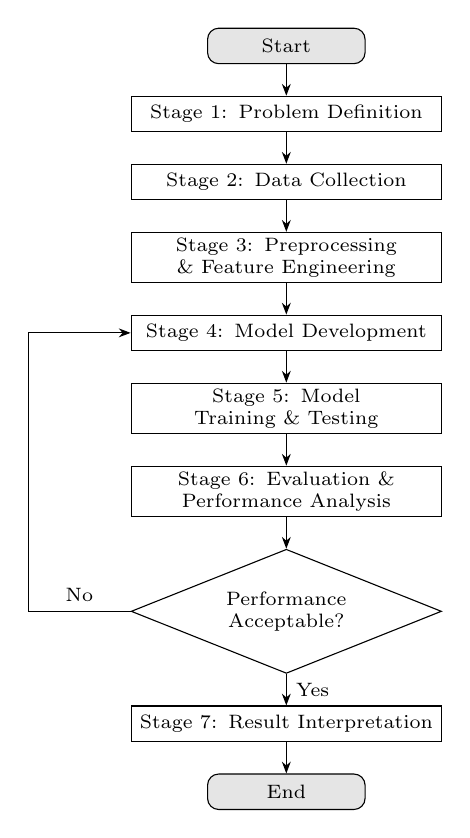
\begin{tikzpicture}[
    node distance=0.4cm,
    every node/.style={font=\scriptsize},
    startstop/.style={rectangle, rounded corners, minimum width=2cm, minimum height=0.45cm, text centered, draw=black, fill=black!10},
    process/.style={rectangle, minimum width=2cm, minimum height=0.45cm, text centered, draw=black, text width=3.8cm, inner sep=2pt},
    decision/.style={diamond, text centered, draw=black, aspect=2.5, inner sep=2pt, text width=2.2cm},
    arrow/.style={-{Stealth[length=1.5mm]}}
]
 
\node (start) [startstop] {Start};
\node (s1) [process, below=of start] {Stage 1: Problem Definition};
\node (s2) [process, below=of s1] {Stage 2: Data Collection};
\node (s3) [process, below=of s2] {Stage 3: Preprocessing \& Feature Engineering};
\node (s4) [process, below=of s3] {Stage 4: Model Development};
\node (s5) [process, below=of s4] {Stage 5: Model Training \& Testing};
\node (s6) [process, below=of s5] {Stage 6: Evaluation \& Performance Analysis};
\node (dec) [decision, below=0.4cm of s6] {Performance Acceptable?};
\node (s7) [process, below=0.4cm of dec] {Stage 7: Result Interpretation};
\node (end) [startstop, below=of s7] {End};
 
\draw [arrow] (start) -- (s1);
\draw [arrow] (s1) -- (s2);
\draw [arrow] (s2) -- (s3);
\draw [arrow] (s3) -- (s4);
\draw [arrow] (s4) -- (s5);
\draw [arrow] (s5) -- (s6);
\draw [arrow] (s6) -- (dec);
\draw [arrow] (dec) -- node[right] {Yes} (s7);
\draw [arrow] (s7) -- (end);
\draw [arrow] (dec.west) -- ++(-1.3,0) node[midway, above] {No} |- (s4.west);
 
\end{tikzpicture}
\caption{Research Methodology Flowchart}
\label{fig:methodology_flowchart}
\end{figure}
 
\subsection{Methodology Explanation}
 
\begin{itemize}
    \item \textbf{Stage 1: Problem Definition} identifies the core limitation that most existing YouTube clickbait detection models rely strictly on metadata features such as titles, view counts, and like ratios while overlooking content-level signals. This stage formulates the research objective: to investigate whether integrating viewer comment sentiment and title-to-transcript semantic similarity into a metadata-based model can improve detection accuracy.
 
    \item \textbf{Stage 2: Data Collection} sources the primary dataset from Vierti's open-source project, which contains approximately 37,000 YouTube video entries that are roughly balanced between the clickbait and non-clickbait classes. Because the original dataset only includes metadata, it is supplemented through a multi-stage filtering funnel to optimize API quota usage and handle rate limitations.
    
    First, transcript availability is validated with youtube-transcript-api. To reduce IP bans and rate limiting, the checker uses a browser-spoofed session and falls back to the official YouTube Data API v3, with mandatory cooldown periods and exponential backoff after repeated failures. Only videos with verifiable transcripts proceed to the next stage. Second, the YouTube Data API v3 commentThreads endpoint is probed per video to confirm comment availability, with API key rotation applied on quota exhaustion to maximize throughput. Videos failing either check are logged and excluded from subsequent processing.
    
    Due to API quota constraints and the computational cost of large-scale extraction, the verification process was halted after processing a sufficient subset of the original corpus. From the ~37,000 entries, videos with verified transcript and comment availability were retained (n = 9,393). The dataset was then rebalanced via random downsampling of the majority class to achieve a 1:1 clickbait-to-non-clickbait ratio, yielding a final working dataset of 5,722 videos (2,861 per class). Because this step keeps only videos that have \emph{both} a public comment section and an available transcript, it introduces a selection bias; its consequences for generalizability are examined in detail in Section IV.
    
    An extraction process was then initiated for the 5,722 confirmed videos. Comment extraction was performed via the YouTube Data API v3 commentThreads.list endpoint, retrieving up to 100 top-level comments per video sorted by relevance. The extractor implements append-mode checkpointing to a running CSV, allowing interrupted runs to resume without duplicating requests. API key rotation is applied automatically on quota exhaustion (HTTP 403), and exponential backoff beginning at 2 seconds with a ceiling of 60 seconds is applied on transient server errors (HTTP 429 and 5xx). Permanent failures (disabled comments, deleted videos) are logged separately and excluded from further processing. Transcript extraction was performed using youtube-transcript-api with a browser-spoofed HTTP session to reduce IP-based rate limiting. Where both manually-created and auto-generated transcripts are available, the manually-created transcript is preferred; otherwise the auto-generated transcript is selected. Requests are spaced with a randomised delay of 4–8 seconds per video. Consecutive IP block events beyond a threshold of five trigger an automatic abort, with blocked video IDs logged to a separate file for retry from an alternative network. The output of this stage, comments.csv and transcripts.csv, is then used in the subsequent preprocessing stage.
 
    \item \textbf{Stage 3: Preprocessing and Feature Engineering} processes the collected data into model-ready features across three categories. First, the baseline features are prepared. Following Vierti's configuration, a Word2Vec model is trained from scratch on the corpus of video titles in the working dataset; it is not a pre-trained or externally downloaded embedding. Training uses lower-cased, whitespace-tokenised titles with a 25-dimensional vector size, a context window of 20, a minimum word count of 1, and 30 epochs, after which each title is represented by averaging the vectors of its tokens. The 25-dimensional size is kept identical to Vierti's original model so that the baseline replication is faithful. Engagement statistics (views, likes, dislikes, and comment counts) are log-scaled with $\log(1+x)$ and then normalized to the $[0,1]$ range using min-max scaling, so that very large counts do not dominate the model. Second, VADER (Valence Aware Dictionary and sEntiment Reasoner) is applied to the extracted comments to compute four aggregate sentiment features per video: the mean and standard deviation of the compound score, and the proportions of positive and negative comments. Third, both the title and transcript of each video are encoded using a pre-trained Sentence-BERT model (all-MiniLM-L6-v2), and a cosine similarity score is computed between the two embeddings to quantify the semantic gap between the title and the actual video content.
 
    \item \textbf{Stage 4: Model Development} establishes the classification models used for comparison. First, Vierti's Support Vector Machine (SVM) classifier is reproduced using only the original metadata features to serve as the baseline benchmark. Second, a Random Forest classifier is developed to handle the combined feature set, which includes the original metadata, comment sentiment scores, and title-to-transcript similarity scores. Random Forest is selected for its resistance to overfitting and its established use in metadata-based clickbait detection \cite{gothankar2022}; whether it remains a good fit once the feature space is dominated by dense Word2Vec dimensions is one of the questions the evaluation is designed to answer. Additionally, an enhanced SVM model is also configured in the same combined feature set, allowing the evaluation to isolate whether performance improvements originate from the new features or the change in the classifier.
 
    \item \textbf{Stage 5: Model Training and Testing} divides the final, balanced dataset into an 80\% training set and a 20\% testing set using stratified sampling to preserve the proportion of clickbait to non-clickbait labels across both subsets. This identical split is maintained across all model configurations (baseline SVM, enhanced SVM, and enhanced Random Forest) to ensure that any performance differences are attributable to the feature set or classifier rather than data variation.
 
    \item \textbf{Stage 6: Evaluation and Performance Analysis} compares all three model configurations on the same held-out test set. Classification performance is measured using accuracy, precision, recall, and F1-score. If the results do not meet expected thresholds or reveal issues such as significant overfitting, the process returns to Stage 4 for hyperparameter adjustment or feature refinement.
 
    \item \textbf{Stage 7: Result Interpretation} benchmarks the enhanced models against the metadata-only baseline to quantify the contribution of the newly introduced features. An error analysis is conducted to identify patterns in false positives and false negatives, and to assess the impact of missing signals such as videos that lack comments or captions. The findings are synthesized into conclusions regarding the effectiveness of content-level features for YouTube clickbait detection, along with recommendations for future work.
\end{itemize}

\section{Results and Discussion}

\subsection{Testing Environment}
All experiments were conducted on a personal computing environment running Windows 11 with an AMD Ryzen 7 5800H processor and 16 GB of DDR4 RAM. No GPU acceleration was used, as all computations were performed on the CPU. The software environment used Python 3.10 with the following key libraries: scikit-learn 1.4 for model training and evaluation, gensim 4.3 for Word2Vec title embeddings, vaderSentiment 3.3.2 for comment sentiment analysis, sentence-transformers 2.6 (model: \texttt{all-MiniLM-L6-v2}) for title-to-transcript semantic similarity, and pandas 2.2 and NumPy 1.26 for data handling. The final data set consisted of 5,722 balanced YouTube video entries (1:1 ratio clickbait:non-clickbait), split into 4,577 training samples and 1,145 test samples using stratified sampling with \texttt{random\_state=42}.

\subsection{Experiment Scenario}
Three model configurations were evaluated to isolate the individual
contributions of the proposed features and the classifier. Table~\ref{tab:model_configs}
summarizes the input, processing pipeline, and output of each configuration.

\begin{table}[htbp]
\caption{Model Configuration Summary}
\label{tab:model_configs}
\centering
\begin{tabular}{|p{1cm}|p{2.5cm}|p{2.0cm}|p{1.5cm}|}
\hline
\textbf{Model} & \textbf{Feature Blocks} & \textbf{Classifier} & \textbf{Purpose} \\
\hline
1 & Block A only (Word2Vec 25-dim, self-trained on our corpus + $\log(1+x)$ engagement) & SVM, RBF (C=3.7, $\gamma$=4.1; from Vierti) & Baseline replication \\
\hline
2 & Block A + B (VADER) + C (SBERT cosine sim) & SVM, RBF (C=10, $\gamma$=scale; tuned) & Feature contribution \\
\hline
3 & Block A + B (VADER) + C (SBERT cosine sim) & Random Forest (n=200, depth unlimited; tuned) & Classifier contribution \\
\hline
\end{tabular}
\end{table}

Each model receives a 34-dimensional feature vector (25 Word2Vec dimensions, 4 log-scaled engagement statistics, 4 VADER comment sentiment aggregates, and 1 SBERT cosine similarity scalar) for Models 2 and 3, and a 29-dimensional vector (Block A only) for Model 1. The identical stratified train/test split is applied across all three configurations to ensure that performance differences are attributable solely to the feature set or classifier, and not to data variation. The evaluation metrics used are accuracy, precision, recall, and F1-score.

\subsection{Experimental Results}
 
Table~\ref{tab:results} presents the classification performance of all
three models on the test set.
 
\begin{table}[htbp]
\caption{Classification Performance Comparison}
\label{tab:results}
\centering
\begin{tabular}{|l|c|c|c|c|}
\hline
\textbf{Model} & \textbf{Accuracy} & \textbf{Precision} & \textbf{Recall} & \textbf{F1-Score} \\
\hline
1. Baseline SVM   & 0.9581 & 0.9645 & 0.9510 & 0.9577 \\
2. Enhanced SVM   & \textbf{0.9616} & 0.9632 & \textbf{0.9598} & \textbf{0.9615} \\
3. Enhanced RF     & 0.9328 & 0.9412 & 0.9231 & 0.9320 \\
\hline
\end{tabular}
\end{table}










\subsection{Analyze and Compare Results}

The results in Table~\ref{tab:results} show a clear difference in performance between the three models. Model 2 (Enhanced SVM) performs the best overall, with an accuracy of 96.16\%, precision of 96.32\%, recall of 95.98\%, and an F1-score of 96.15\%. This is slightly better than Model 1 (Baseline SVM), which achieved 95.81\% accuracy and a 95.77\% F1-score. Model 3 (Enhanced Random Forest) performed the worst of the three despite using the same features as Model 2, with only 93.28\% accuracy and a 93.20\% F1-score.

The improvement from Model 1 to Model 2 shows that adding VADER comment sentiment and Sentence-BERT title-to-transcript similarity does help the classifier. The biggest difference is in recall, which went up from 95.10\% to 95.98\%. A higher recall means the model catches more actual clickbait videos that the baseline would have missed. This makes sense because negative comment sentiment reflects viewer disappointment, which is common when a video turns out to be misleading \cite{elyashar2022}, and a low similarity between the title and the transcript shows that the video does not actually deliver what the title promises \cite{varshney2021, ahmadi2023}. Looking at the confusion matrix, Model 2 also reduced false negatives from 28 to 23 compared to Model 1.

That said, whether this improvement justifies its cost is a fair question. The difference in accuracy between Model 1 and Model 2 is only about 0.35\%, and the F1-score only improved by 0.38\%. To get that small gain, the pipeline needed comment data from the YouTube Data API, which has strict daily quota limits and required rotating multiple API keys. It also needed transcripts retrieved using cookie spoofing to avoid IP blocks, and then encoded using Sentence-BERT, which is much more computationally expensive than the Word2Vec embeddings used in the baseline. For a research study where the goal is to test whether these features help, this tradeoff is acceptable. But in a real-world system that needs to process videos quickly or at large scale, the added complexity may not be justified by such a small performance gain. In that case, Model 1 would likely be the more practical choice.

Model 3's weaker performance also merits explanation. Random Forest is generally effective on datasets with mixed feature types \cite{gothankar2022}, but here the feature set is dominated by 25 continuous Word2Vec dimensions, which are not well suited to axis-aligned tree splits. An SVM with an RBF kernel handles this kind of dense, continuous data better because it can form more flexible decision boundaries \cite{vierti2019}. The limitation therefore appears to lie in the model class itself rather than in its tuning.

On the topic of model parameters, the specific values $C$=3.7 and $\gamma$=4.1 used for the baseline (Model 1) are not arbitrary choices and are not scikit-learn defaults: they are the exact hyperparameters reported by Vierti \cite{vierti2019}, and they were reused unchanged so that Model 1 is a faithful replication of that baseline rather than a newly tuned model. Because the enhanced models operate on a larger 34-dimensional feature space, keeping hyperparameters that were tuned for the original feature space would not be appropriate, so Models 2 and 3 were each re-tuned on their own feature space using a grid search with five-fold cross-validation that optimized the F1-score. Vierti's original values were deliberately included in the search grid so that they remained reachable if they turned out to be optimal. For Model 2 the search selected $C$=10 with $\gamma$=scale (scikit-learn's variance-based heuristic, $\gamma = 1/(n_\text{features}\cdot\text{Var}(X))$) rather than Vierti's values, which is expected given the larger feature space. For Model 3 it selected 200 trees with unlimited depth and a minimum split size of 2. Model 3 still underperformed after this tuning, which suggests the problem is not the hyperparameters but the model type itself.

Data collection was among the principal challenges of this study. Transcript retrieval was difficult because YouTube throttles requests once too many are issued in a short period; to mitigate this, requests were sent through a cookie-backed browser session so that they more closely resembled ordinary user traffic. Even so, extraction was blocked on several occasions and had to be resumed from different networks. Comment extraction through the official YouTube Data API was similarly slowed by daily quota limits, which made it necessary to rotate several API keys. These constraints reduced the dataset from roughly 37,000 videos to the 9,393 that had both a retrievable transcript and available comments, which were then balanced by random downsampling of the majority class to 5,722 (2,861 per class). It is important to be clear that this reduction was forced by practical data-collection constraints --- API quotas, rate limiting, and IP blocking --- and not by any property of the videos themselves, so it should be treated as a limitation of this study rather than a deliberate sampling design. The reduction has two main effects. First, it lowers the volume of training data, which reduces statistical power and can make the reported metrics more sensitive to the particular train/test split; nonetheless, 5,722 class-balanced samples remain sufficient to train and fairly compare the three configurations. Second, and more importantly, it introduces a selection bias: by construction the working dataset contains only videos that have \emph{both} a public comment section and an available transcript, which systematically excludes videos with comments disabled, videos without captions, and many non-English or music-only videos. If these excluded videos are not distributed evenly across the clickbait and non-clickbait classes, the class balance and feature distributions of the filtered set may differ from those of YouTube as a whole. The verification funnel already shows such an asymmetry: of the videos checked, only about 31\% of clickbait items had both a transcript and an open comment section, against roughly 68\% of non-clickbait items, which is consistent with clickbait creators being more inclined to disable comments to hide viewer backlash. Consequently, the high accuracy reported here should be read as accuracy on the population of \emph{commentable and transcribable} videos, and the model's generalization to the full range of YouTube videos remains an open question that future work should test on a less restrictively filtered sample.

There is also a concern about transcript quality. When no manually-created transcript was available, the auto-generated one from YouTube was used instead. These are produced by speech recognition software and can contain errors, especially in videos with accents, fast talking, or technical words. These errors can affect the Sentence-BERT similarity score in unpredictable ways, since the transcript no longer accurately reflects what was actually said. A misleading video might get a high similarity score by accident, or a normal video might get a low one due to poor transcription quality. Measuring exactly how much this affects the results would require manually checking the transcripts, which was not done in this study and is left as something to address in future work.

Comparing these results to previous studies, Model 2 (F1=96.15\%) performs better than metadata-only approaches found in the literature. Gothankar et al. \cite{gothankar2022} suggested that comparing titles to transcripts could be useful but never tested it; the results here show that this approach is effective in practice. Ahmadi and Chowanda \cite{ahmadi2023} showed that title-to-content similarity works well for detecting clickbait in news articles, and this study shows it can also be applied to YouTube videos using auto-generated transcripts. The improvement in recall from Model 1 to Model 2 also supports the finding by Elyashar et al. \cite{elyashar2022} that comment reactions are a useful signal, though the effect is smaller here because the VADER features are mixed in with many other stronger features. The overall accuracy is slightly lower than the 98\% reported by Bronakowski et al. \cite{bronakowski2023}, but that study was done on news headlines, which are simpler and more consistent than YouTube titles. Video content is more varied and harder to classify. Overall, the results here are in line with what other studies have found, which is that using content-aware features alongside metadata leads to better detection \cite{bronakowski2023, bajaj2024}.


























\section{Conclusion}

This study set out to test whether two content-level signals---the sentiment of viewer comments and the semantic similarity between a video's title and its transcript---can improve a metadata-based clickbait detector on YouTube. Starting from Vierti's SVM baseline, we added VADER sentiment features and a Sentence-BERT title-to-transcript similarity score, and compared three configurations on the same balanced subset of 5,722 videos: the baseline SVM, an enhanced SVM, and an enhanced Random Forest.

The added features did help, but only modestly. The enhanced SVM was the best model at 96.16\% accuracy and 96.15\% F1, against 95.81\% accuracy for the metadata-only baseline. The clearest gain was in recall: false negatives fell from 28 to 23, meaning the enhanced model caught more of the clickbait the baseline missed. This is consistent with the idea that negative viewer comments and a weak title-to-transcript match are useful indicators of misleading content. The Random Forest, despite using the same features, was the weakest of the three at 93.28\% accuracy; the feature space is dominated by 25 dense Word2Vec dimensions, which suit the margin-based SVM far better than tree-based splitting. The improvement therefore came from the new features rather than from changing the classifier.

These results should be read with two limits in mind. First, the gain in accuracy is small relative to the cost of collecting comments and transcripts at scale, so the metadata-only baseline may remain the more practical choice for a production system. Second, the working dataset contains only videos that have both a public comment section and an available transcript, so the reported accuracy applies to that population rather than to YouTube as a whole, and the auto-generated transcripts add noise to the similarity score that this study did not quantify.

Future work should test the same features on a larger and less restrictively filtered sample, measure how much auto-generated transcript errors affect the similarity feature, and explore stronger title and content encoders or a more direct way of combining the comment signal so that it is not diluted by the metadata features.

% To add citations, please use the bibliography.bib
\bibliographystyle{IEEEtran}
\bibliography{bibliography}

\end{document}